\chapter{Poprawno�� warto�ci sygna��w w punkcie pracy}

\section{Poprawno�� sygna��w}
W celu sprawdzenia poprawno�ci sygna��w $U_{pp}$ oraz $Y_{pp}$ obiekt zosta� pobudzony sygna�em o warto�ci $U_{pp}$. Warto�ci sygna��w w punkcie pracy s� poprawne, je�li sygna� wyj�ciowy przyjmie warto�� $Y_{pp}$.

\begin{figure}[tb]
\centering
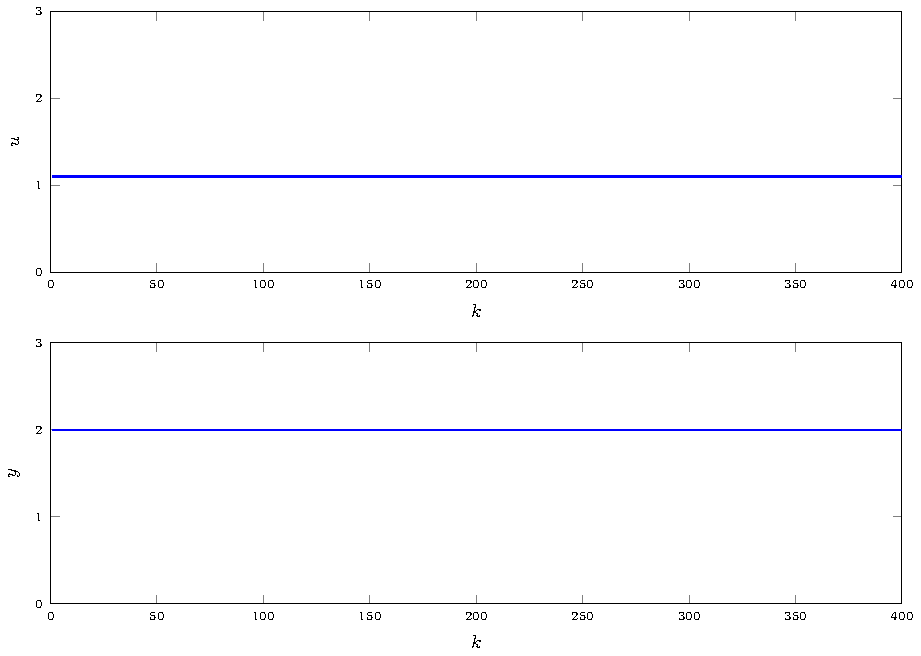
\includegraphics[scale=1]{rysunki/zapisz_pdf/zad1}
\caption{Warto�ci sygna��w w punkcie pracy}
\end{figure}

\section{Wnioski}
Na podstawie rysunku wida�, �e dla sta�ej warto�ci sygna�u steruj�cego $U_{pp}$ wyj�cie obiektu przyjmuje sta�� warto��, r�wn� $Y_{pp}$. Jest to dow�d na to, �e warto�ci sygna��w wejsciowego i wyj�ciowego w punkcie pracy s� poprawne.

\section{Implementacja}
Do przeprowadzenia eksperymentu wykorzystany zosta� skrypt \verb+zad1.m+.